\documentclass[a0paper,portrait]{baposter}
\usepackage{cite,url,amsthm,footmisc,bm}
\usepackage{amsmath,graphicx,amssymb,algorithm,algorithmic,subfigure,epsfig,multirow,threeparttable,booktabs,bm,mathdots,tabularx}
\usepackage[font=small,labelfont=bf]{caption} % Required for specifying captions to tables and figures
\usepackage{booktabs} % Horizontal rules in tables
\usepackage{relsize} % Used for making text smaller in some places
\usepackage{float}
\usepackage{natbib}
\usepackage{etoolbox}
\patchcmd{\thebibliography}{\section*{\refname}}{}{}{}

\graphicspath{{images/}} % Directory in which figures are stored

\definecolor{bordercol}{RGB}{40,40,40} % Border color of content boxes
\definecolor{headercol1}{RGB}{186,215,230} % Background color for the header in the content boxes (left side)
\definecolor{headercol2}{RGB}{80,80,80} % Background color for the header in the content boxes (right side)
\definecolor{headerfontcol}{RGB}{255,255,255} % Text color for the header text in the content boxes
\definecolor{boxcolor}{RGB}{255,255,255} % Background color for the content in the content boxes

\def\bibfont{\footnotesize}

\begin{document}

\background{ % Set the background to an image (background.pdf)
  \begin{tikzpicture}[remember picture,overlay]
    
  \end{tikzpicture}
}

\begin{poster}{
    grid=false,
    borderColor=bordercol, % Border color of content boxes
    headerColorOne=headercol2, % Background color for the header in the content boxes (left side)
    headerColorTwo=headercol1, % Background color for the header in the content boxes (right side)
    headerFontColor=headerfontcol, % Text color for the header text in the content boxes
    boxColorOne=boxcolor, % Background color for the content in the content boxes
    headershape=roundedright, % Specify the rounded corner in the content box headers
    headerfont=\Large\sf\bf, % Font modifiers for the text in the content box headers
    textborder=rectangle,
    background=user,
    headerborder=open, % Change to closed for a line under the content box headers
    boxshade=plain
    }{}
    {Calculation of Auger recombination thresholds in narrow gap HgCdTe based QW heterostructures} % Poster title
    {\vspace{1em} Kulikov N.S., Rumyantsev V.V., Zholudev M.S., Utochkin V.V., Morozov S.V.  \\ % Author names
    {\smaller neilkulikov@gmail.com}} % Author email addresses
    {
\includegraphics[scale=0.75]{logo.png}}

    \headerbox{Abstract}{name=intro,column=0,row=0}{
        Auger recombination is a three-particle threshold process. It can be considered 
        that as a result of the recombination of two particles, the third one acquires 
        high energy and momentum. This effect reduces the population inversion and heats 
        up charge carriers, which leads to its competition with the process of 
        stimulated radiation. An obvious way to reduce the rate of such a process is to 
        increase the Auger threshold energy \cite{Rumyantsev:IOP:2018}. It can be defined as the total kinetic energy 
        of the initial particles.
    }

    \headerbox{Analityc relations}{name=anal,column=0,row=0,below=intro}{
        A problem can be defined mathematically. It is proposed to consider two different 
        options: CCHC \& HHCH processes. Also we can minimize the final state energy,
        it linearly depends on $\varepsilon_{th}$.

        \begin{equation}
            \begin{array}{l}
                \label{gfunc}
                \varepsilon_{th} = \min_{\vec{k}_1, \vec{k}_2, \vec{k}_3} K (\vec{k}_1, \vec{k}_2, \vec{k}_3);\\
                \begin{cases}
                    K  = \varepsilon_f(\vec{k}_1 + \vec{k}_2 - \vec{k}_3) - \beta \cdot \varepsilon_g;\\
                    \beta = \begin{cases}
                                1   & \text{CCHC}\\
                                2   & \text{HHCH}
                            \end{cases};\\
                    \varepsilon_1(\vec{k}_1) + \varepsilon_2(\vec{k}_2) - \varepsilon_3(\vec{k}_3) = \varepsilon_f(\vec{k}_1 + \vec{k}_2 + \vec{k}_h);
                \end{cases}
            \end{array}
        \end{equation}

        A necessary condition for the minimum is the coincidence of the group velocities of the particles:

        \begin{equation}
            \nabla \varepsilon_1(\vec{k}_1) = \nabla \varepsilon_2(\vec{k}_2) = \nabla \varepsilon_h(\vec{k}_h);
        \end{equation}

        In most cases, this leads to the fact that the CCHC process is dominant.
    }

    \headerbox{Algorithm description}{name=algo,column = 0,below=anal}{
        The energy-momentum law can be calculated for HgCdTe heterostructures in the Kane 8x8 
        model \cite{Zholudev:PRB:2012}. It can be interpolated with Akima cubic splines.
        This trick provides enough smoothness and also helps to avoid parasitic oscillations.

        The function \ref{gfunc} can be optimized with the Lagrange method. Starting points can be 
        selected on sites with the same derivative \& second derivative sign. This fact ensures 
        finding the required points.

        The maximum threshold energy is considered limited by temperature \cite{Rumyantsev:IOP:2018}:
        \begin{equation}
            \varepsilon_{th,max} = 2T;
        \end{equation}


    }


    \headerbox{References}{name=refs,column = 0,row = 2,above=bottom}{
            \bibliographystyle{plain}
            \bibliography{Bibliography}
            %\printbibliography[heading=none]
        }


    \headerbox{Experimental spectrum}{name=spec,column=1,span=2}{
                \centering{
                    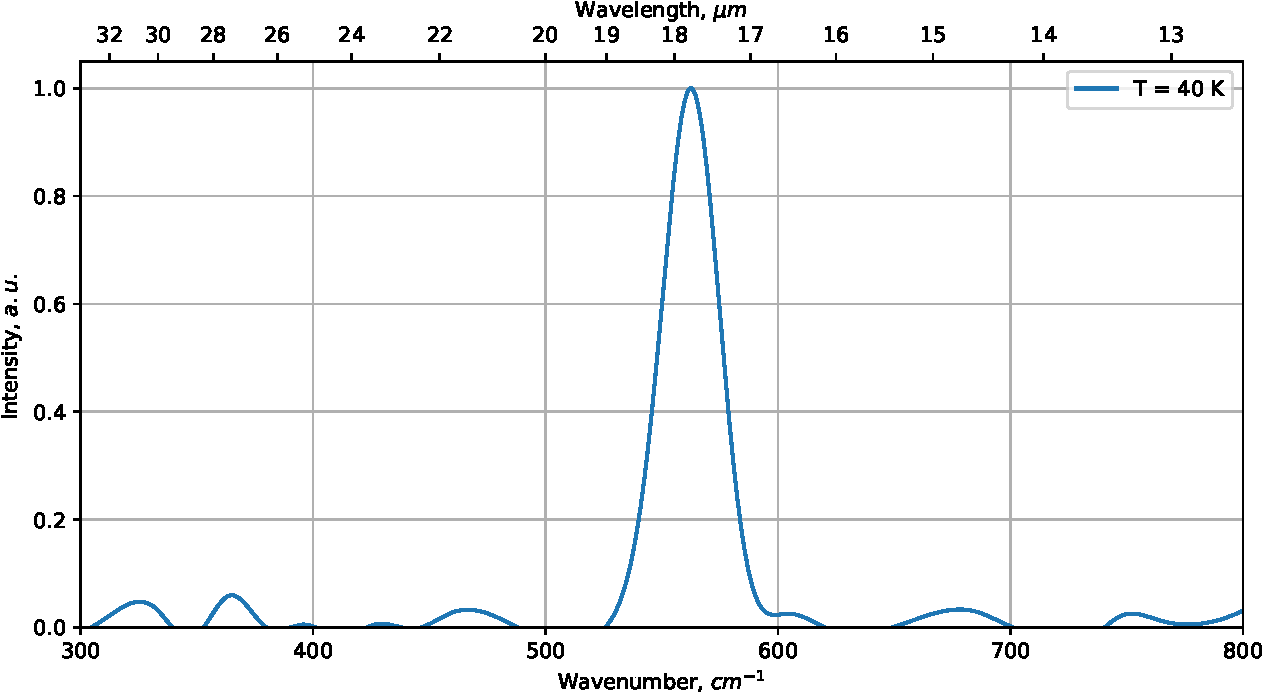
\includegraphics[width=0.9\linewidth]{new_18um_spectre.pdf}
                    \captionof{figure}{\label{spec}Stimulated emission spectra}
                }
                }
    \headerbox{Auger threshold energy vs. barriers}{name=tvsb,column=1,span=2,below=spec}{
                \centering{
                    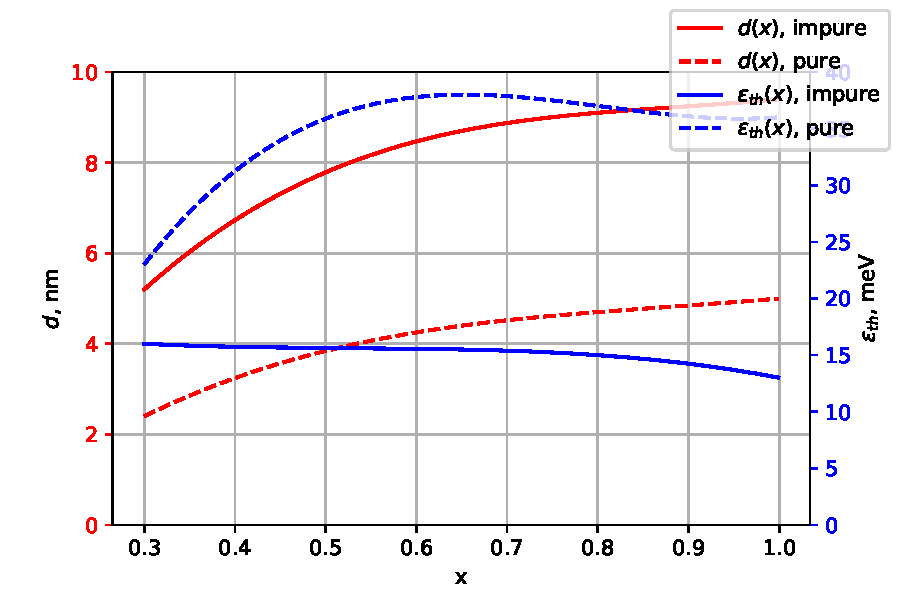
\includegraphics[width=0.9\linewidth]{de_vs_x.pdf}
                    \captionof{figure}{\label{tvsb}The dependence of Auger-threshold energy 
                    and required QW thickness on the concentration of Cd 
                    in barriers with fixed temperature and $\varepsilon_g$.}
                }
    }
    \headerbox{Comparison at various Cd\%}{name=pimp,column=1,span=1,below=tvsb,above=bottom}{
                \begin{minipage}[h]{1.\linewidth}
                    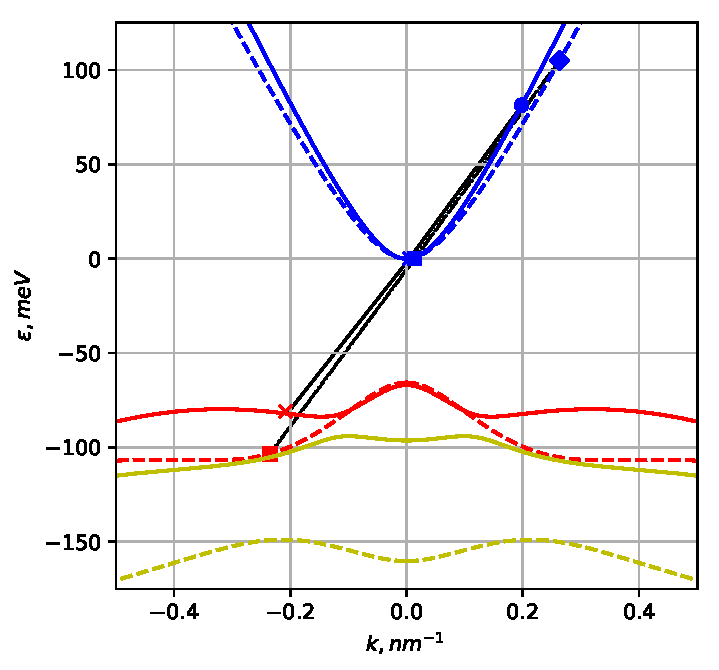
\includegraphics[width=\linewidth]{18um_p_vs_i.pdf}
                    \captionof{figure}{\label{pimp}Threshold Auger processes 
                    in $Hg_{1-x} Cd_x Te$ QWs for $x = 0.1,~x=0$.}
                \end{minipage}
    }
                
    \headerbox{Discussion}{name=spec,column=2,span=1,below=tvsb}{ 
        We consider the structure of the composition $Hg_{0.9} Cd_{0.1}Te/Cd_{0.65} Hg_{0.35} Te$
        with 10 unrelated quantum wells 8.7 nm thick. It allows to observe stimulated radiation 
        with $\lambda \approx 18~\mu m$ close to 40 K.

        On Fig. \ref{spec} we can see the SE spectre at T = 40 K.
        Continuous lines are responsible for the structure described
        above, shaded lines are responsible for the structure without 
        cadmium in the QWs.
        We can investigate the effect of cadmium content in quantum wells 
        on threshold energy. As it can be shown, lower concentration of Cd
        reduces side maximums and increases threshold energy.
        
        It would be interesting to investigate the dependence of the threshold 
        energy on the composition of the barriers. As it can be shown in Fig. \ref{tvsb},
        there is a severe maximum for the case of pure quantum wells.
    }
\end{poster}
\end{document}